\section{SNCF \& VSC Technologies}
\subsection{Le Groupe SNCF}

\subsubsection{Présentation Générale}
La Société nationale des chemins de fer français (SNCF) est l'entreprise ferroviaire publique française, officiellement créée le 1er janvier 1938 en application du décret-loi du 31 août 1937.
Elle est notamment présente dans les domaines du transport de voyageurs, du transport de marchandises et réalise la gestion, l'exploitation et la maintenance du réseau ferré national dont elle est propriétaire.

La SNCF est donc une entreprise ferroviaire « intégrée » : elle exerce à la fois le métier d'exploitant (voyageurs et marchandises) et celui de gestionnaire d'infrastructure ferroviaire.

La Société nationale des chemins de fer français est devenue un établissement public à caractère industriel et commercial en 1983, alors qu'elle était auparavant une société anonyme d'économie mixte.

En 2015, le réseau ferré national propriété de SNCF Réseau compte environ 30,000 kilomètres de lignes dont 15 687 km de lignes électrifiées et 2 024 km de lignes à grande vitesse.

Chaque jour, elle fait circuler 15 000 trains de fret et de voyageurs et transporte plus de cinq millions de voyageurs. Par son volume d'activité et la taille de son réseau, c'est la troisième entreprise ferroviaire européenne, après la Deutsche Bahn et les chemins de fer russes.

Elle détient des participations majoritaires ou totales dans des sociétés de droit privé regroupées dans le groupe SNCF et dont la tutelle de l'État est exercée par la Direction générale des infrastructures, des transports et de la mer du ministère de l'écologie, du développement durable et de l'énergie.

En 2014, la SNCF a enregistré un résultat net de 605 millions d'euros (contre une perte nette de 180 millions d'euros en 2013).

Le reste du groupe SNCF, qui a réalisé 7,1 milliards d'euros de chiffre d'affaires en novembre 2009, intervient dans les domaines suivants : logistique et transport routier de marchandises, transport routier de voyageurs (Keolis), liaison maritime (SeaFrance), ingénierie (EFFIA, INEXIA, commerce en ligne (Voyages-sncf.com), billet-tique (RITMx). Le groupe possède aussi des participations dans des sociétés ferroviaires et gestionnaires d'infrastructure portuaire partagées avec d'autres partenaires comme Eurostar, Thalys, Elipsos, Lyria et Nuovo Trasporto Viaggiatori.

\subsubsection{Organisation}
Depuis le 1er janvier 2015,
la SNCF est constituée de trois établissements publics à caractère industriel et commercial (EPIC, lexique.\ref{lexi:epic}) (fig.\ref{fig:sncf_epic}) :

\begin{itemize}
 \item un ÉPIC SNCF, qui prend en charge le pilotage global du groupe;
 \item un ÉPIC SNCF Réseau, qui gère, exploite et développe le réseau ferré français;
 \item un ÉPIC SNCF Mobilités, pour le transport de voyageurs et de marchandises.
\end{itemize}
et cinq « métiers »:
\begin{itemize}
 \item SNCF Réseau;
 \item SNCF Voyageurs;
 \item SNCF Logistics;
 \item SNCF Immobilier;
 \item SNCF Keolis.
\end{itemize}

Elle possède aussi de nombreuses filiales aussi bien de droit public que de droit privé qui forment le groupe SNCF.

\begin{figure}[ht]
 \centering
 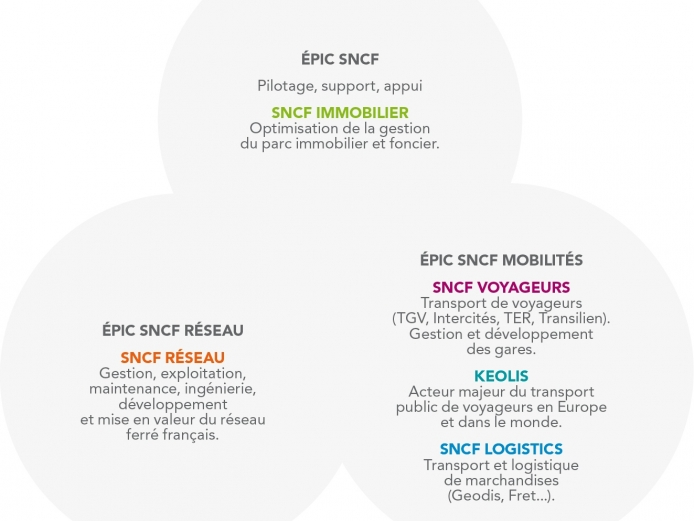
\includegraphics[width=0.9\textwidth]{sncf_epic}
 \caption{Epic SNCF}
 \label{fig:sncf_epic}
\end{figure}

\subsection{Le Groupe VSC \& Rail Europe}
\subsubsection{Présentation Générale}

Le Groupe VSC et Rail Europe, filiale du Groupe SNCF qui se situe dans l'EPIC "SNCF Mobilités", dirigée par Franck Gervais, est un acteur majeur du tourisme, expert de la distribution du train mais aussi de la vente des billets d'avions, de séjours, location de voitures et chambres d'hôtel, en France et en Europe. En 2015, son volume d’affaires atteint 4,1 milliards d’euros, en recul de 1,4\% par rapport à 2015 en vendant 86 millions de voyages, en croissance de 4,4\%. L’innovation demeure un axe central et exprime la capacité de Voyages-sncf.com à répondre aux nouveaux usages de ses clients. Aujourd’hui, en France, Voyages-sncf.com est le premier site d’e-commerce et la première agence de voyages en ligne ; le groupe rassemble 1200 collaborateurs dans le monde dont 40\% à l'international (130 en Europe et 350 hors Europe).

En 2000, le site internet Voyages-sncf.com (fig.\ref{fig:vsct_site}) est lancé sur le périmètre France. L’entreprise est à l’époque le distributeur unique des billets de train SNCF, et a pour objectif de transformer son site en portail de voyages offrant des produits et services complémentaires au train. L’année suivante, Voyages-sncf.com forme une joint-venture avec l’américain Expedia et devient une agence de voyage globale. L’entreprise poursuit alors son développement en France, tout en nourrissant une ambition internationale.

\begin{figure}[ht]
 \centering
 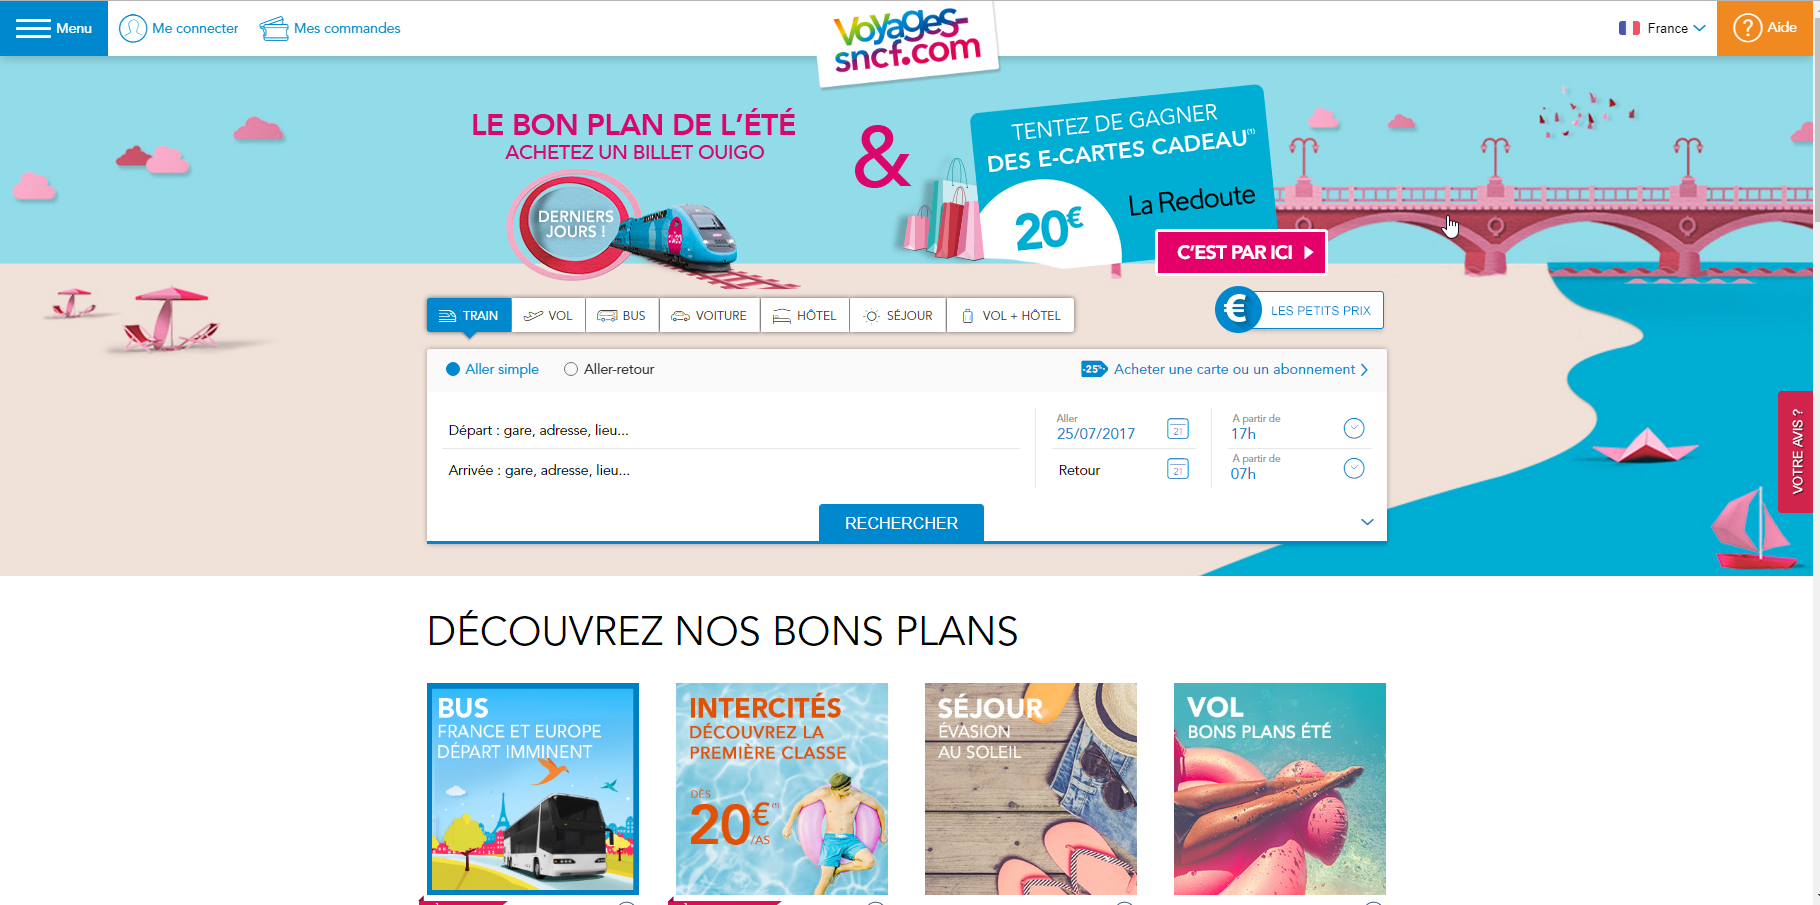
\includegraphics[width=0.9\textwidth]{vsct_site}
 \caption{Le site de Voyages Sncf}
 \label{fig:vsct_site}
\end{figure}

Pour répondre aux enjeux de la distribution du voyage et aux nouveaux comportements d’achats, le groupe VSC offre à ses clients mondiaux un réseau puissant, souple et adapté à leurs besoins. Il couvre plus présent dans 11 pays européens et 45 dans le reste du monde via un total de 67 sites internet et mobiles, 4 boutiques et un service de call-center. Afin de répondre aux enjeux spécifiques du marché B2B, le site Voyages-sncf.eu a été lancé en Europe en 12 langues (hors France).
Le site recense plusieurs transporteurs tels que SNCF, TER, Eurostar, Thalys, TGV Lyria ; 3 compagnies de bus, 400 compagnies aériennes ; 280 000 hôtels référencés ; plus de 25 000 offres de séjours ; 30 loueurs de voitures, etc.

\begin{figure}[ht]
 \centering
 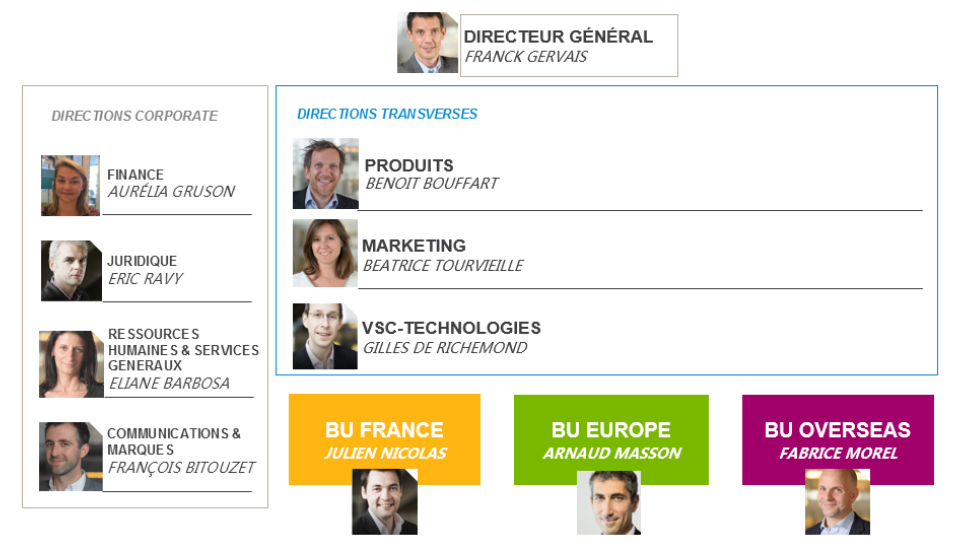
\includegraphics[width=0.9\textwidth]{vsc_organisation}
 \caption{VSC: Organisation}
\end{figure}

Le groupe va lancer la nouvelle marque OUI.sncf le 7 décembre 2017.
Ce changement fera évoluer la plateforme transactionnelle.

\subsubsection{Organisation}
L'organisation du Groupe VSC est basée sur 3 BU’s :
Trois BU’s transport sur trois zones géographiques : France, Europe, et Overseas.
L’outil industriel et nos grandes expertises sont mutualisées dans des équipes dédiées travaillant pour ces trois BU’s : les Directions Produits, la Technologie et le Marketing. Enfin, des Directions corporate assistent l'ensemble.

Le Groupe VSC est la filiale de Distribution Digitale de Voyages SNCF.
Voyages SNCF fait partie de Voyageurs, l'une des branches de l'EPIC SNCF Mobilités. 
Voyages SNCF assure le transport ferroviaire longue distance et à grande vitesse de plus de 130 millions de personnes par an dans toute l’Europe, à bord des 500  rames TGV, iDTGV, Ouigo, Eurostar, Thalys, Lyria et Ellipsos. Ouibus fait également partie de Voyages SNCF.

\subsubsection{VSC Technologies (VSCT)}
VSC Technologies, entité du Groupe Voyages-sncf.com,
est en charge de la partie informatique du premier site public de e-commerce français.
VSC Technologies propose des solutions informatiques dans une logique éditeur,
développe des offres sur mesure pour répondre aux besoins de ses clients (SNCF, Eurostar, IDTGV...) 

\begin{figure}[ht]
 \centering
 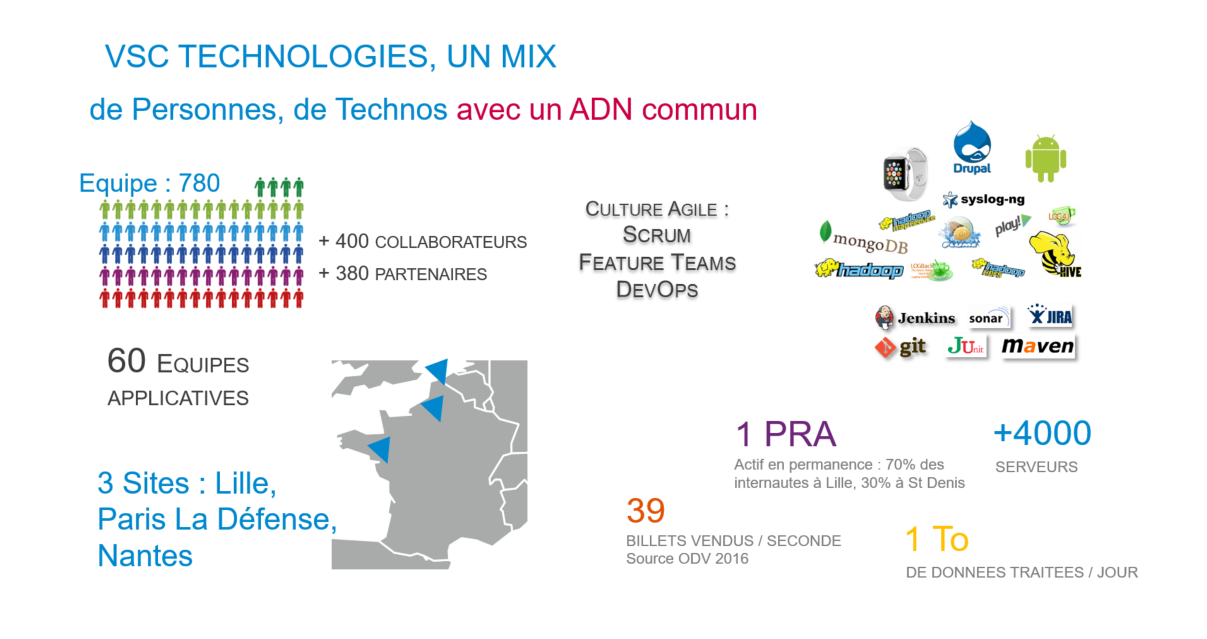
\includegraphics[width=0.9\textwidth]{vsct}
 \caption{VSC Technologies: Un mix}
 \label{fig:vsct}
\end{figure}

\clearpage
